\hfill\\
\section{Methodology}\hfill

In this work, we introduce a machine learning approach that incorporates jets and tracks to quantify $E_{frac}$ and $M_{frac}$ of jets. We define this problem as a regression task: $f(\mathcal{J},\mathcal{T})[\theta] \Rightarrow M_{frac}$ and $g(\mathcal{J},\mathcal{T})[\psi] \Rightarrow E_{frac}$, where $\theta$ and $\psi$ are model parameters. We consider jet tensor $\mathcal{J} \in \mathbb{R}^{N_J \times x}$ with features: $[p_T,\eta,\phi,m]$, and track tensor $\mathcal{T} \in \mathbb{R}^{N_J \times N_T \times y}$ with features: $[p_T,\eta,\phi,m,d_0,z_0]$\footnote{Transverse, $d_0$, and longitudinal, $z_0$, distance to primary vertex when track is extrapolated to beam line using parameterized estimation}, where $x$ is jet feature dimensions, $y$ is track feature dimensions, $N_J$ is the total number of jets in an event, $N_T$ is the total number of tracks in an event. We depict the overall architecture of the proposed model in Figure~\ref{fig:Model}. The goal of this work is to extract rich contextual information that exists in track features, $\mathcal{T}$, to reinforce jet features, $\mathcal{J}$, using transformer-based encoder to capture correlations within and between these inputs.

\begin{figure}[h]
\centering
  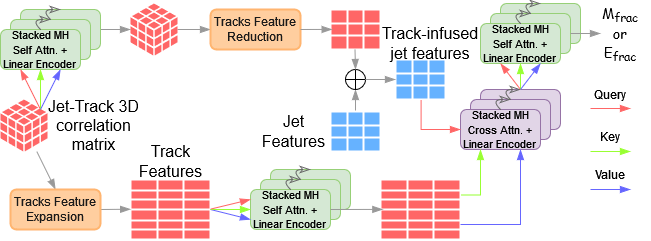
\includegraphics[width=1\linewidth]{PAKDD25-architecture.png}
\caption{Track Tensor, $\mathcal{T}$, in red and Jet Tensor, $\mathcal{J}$, in blue.}
\label{fig:Model}
\end{figure}


\subsection{Transformer Encoder} \hfill

The core building block of our model is a transformer encoder, which operates on inputs \(Q\) (query), \(K\) (key), and \(V\) (value). First, the encoder uses Layer Normalization to initialize inputs: $\mathbf{Q} = \text{LN}(Q), \mathbf{K} = \text{LN}(K), \mathbf{V} = \text{LN}(V)$. Second, scaled-dot product attention is used to calculate the attention weights and extract correlations: $\text{Attention}(\mathbf{Q}, \mathbf{K}, \mathbf{V}) = \text{softmax}\left(\frac{\mathbf{Q} \mathbf{K}^\top}{\sqrt{d_E}}\right) \mathbf{V}$. In practice, multi-head attention, MHA, is used for deeper learning where $num\_heads=8$. Third, a residual connections is used to generate the context vector: $\mathbf{Q}_\text{Context} = \mathbf{Q} + \text{MHA}(\mathbf{Q}, \mathbf{K}, \mathbf{V})$. Fourth, a feed-forward network and additional skip connection is used to produce the updated representation of the input query: $\mathbf{Q}_\text{Output} = \mathbf{Q}_\text{Context} + \text{FFN}(\mathbf{Q}\text{Context})$. This encoder block can be stacked numerous times to iteratively update the query with various key-value pairs. Therefore, the two types of encoder used by the model can be summarized as self-encoders and cross-encoders for input sets $\mathbb{X}$ and $\mathbb{Y}$:

\begin{equation}
    \text{Self-Encoder}(\mathbb{X},\mathbb{X},\mathbb{X}) = \mathbb{X}' \quad \text{Cross-Encoder}(\mathbb{X},\mathbb{Y},\mathbb{Y}) = \mathbb{X}'
\end{equation}

\subsection{Local Track Enrichment of Jets}
\label{sec:trk-agg}

The first method to enrich $\mathcal{J}$ with $\mathcal{T}$ is depicted in the upper branch of Figure \ref{fig:Model} through a 3-step process: (1) self-encoder is applied to $\mathcal{T}$ to capture local correlations between tracks, (2) reduction operation is applied, and (3) reduced track tensor is concatenated with jet tensor to achieve an updated representation of jets. These operatoins are summarized as:

\begin{align}
  \mathcal{T}' &= \text{Self-Encoder}(\mathcal{T},\mathcal{T},\mathcal{T}) \\
  \mathcal{T}_\text{reduced}&=\sum\limits_{dim=1} \mathcal{T}' \\
  \mathcal{J}_\text{local}&=\mathcal{J} \oplus \mathcal{T}_\text{reduced}
\end{align}


\subsection{Global Track Enrichment of Jets} \hfill

The second method to enrich $\mathcal{J}$ with $\mathcal{T}$ is depicted in the lower branch of Figure \ref{fig:Model} through a 3-step process: (1) feature expansion is applied to flatten $\mathcal{T}$, (2) self-encoder is applied to $\mathcal{T}$ to capture global correlations between tracks, and (3) cross-encoder is applied to $\mathcal{J}$ and $\mathcal{T}$ to capture correlations between jets and all tracks.

\begin{align}
  \mathcal{T}_\text{flat}&=\text{Flatten}(\mathcal{T},dim=1) \\
  \mathcal{T}_\text{flat}' &= \text{Self-Encoder}(\mathcal{T}_\text{flat},\mathcal{T}_\text{flat},\mathcal{T}_\text{flat}) \\
  \mathcal{J}_\text{global} &= \text{Cross-Encoder}(\mathcal{J}_\text{local},\mathcal{T}_\text{flat}',\mathcal{T}_\text{flat}') \\
\end{align}

A final self-encoder between jets is used to provide full event context: $\mathcal{J}_\text{final} = \text{Self-Encoder}(\mathcal{J}_\text{global},\mathcal{J}_\text{global},\mathcal{J}_\text{global}) $. These final jet embeddings, \(\mathcal{J}_{\text{final}}\), are passed through a regression layer with sigmoid activation to predict $E_{\text{frac}}$ and $M_{\text{frac}}$.

\subsection{Learning Objective}\hfill

The model is trained on the diHiggs simulated dataset, described in Section \ref{Dataset} depicted in Figure \ref{fig:HLLHC}, using Efrac and Mfrac as targets, described in Section \ref{JetLabels} depicted in Figure \ref{fig:Labels} using a Mean Squared Error loss function. In practice, each encoder block is stacked three times to give the model more learnable parameters, $\sim$4.1M,  to achieve a deeper representation of jets. During the training process, the learning rate is scheduled to decay by a factor of 0.1 after the 25th epoch which noticeably helped descend the noisy loss landscape. The AdamW optimizer is used to prevent overtraining using weight decay, and Mean Squared Error was used as the loss function. The model converged after training 50 epochs on an NVIDIA RTX 3090.


%%%%%%%%%%%%%%%%%%%%%%%%%%
%%% Multi-Line Comment %%%
%%%%%%%%%%%%%%%%%%%%%%%%%%
\iffalse
\subsection{Model Architecture}\hfill

Four transformer encoder stacks are used to enrich each tensor -- $\mathbb{J},\mathbb{T}_{jet},\mathbb{T}_{jet}$ -- with context from the event. Each encoder follows the NormFormer [*] architecture by (... et al). NormFormers consists of LayerNorms, LN(), multi-head attention, MHA(), skip connections, + operator, feed-forward network, FFN, which consists of a linear layer and a GELU activation function. These layers are the components of each encoder block.


First, each jet is enriched with associated tracks. Since each jet only carries four features, $p_T, \eta, \phi, m$, tracks within a radius of $\Delta R = 0.4$ are used in the first encoder stack to achieve a rich representation of each jet.

\begin{align}
    \mathbb{T}_{context} &= \mathbb{T}_{jet} + LN(MHA(LN(\mathbb{T}_{jet}), LN(\mathbb{T}_{jet}), LN(\mathbb{T}_{jet}))) \\
    \mathbb{T}_{embed} &= \mathbb{T}_{context} + FFN (\mathbb{T}_{context}) \\
    \mathbb{T}_{aggregated} &= \sum_{dim=1} \mathbb{T}_{embed} \\ 
    \mathbb{J}_{enriched} &= FFN(\mathbb{J} \mathop{\oplus}_{dim=1} \mathbb{T}_{aggregated})
\end{align}
$\mathbb{T}_{jet}$, $\mathbb{T}_{context}$, and $\mathbb{T}_{embed}$ all have shape $N_{jet} \times N_{trk} \times E_{dim}$. Then the summation operator reduces the $N_{trk}$ dimension which will then match the dimension of $\mathbb{J}$ with shape $N_{jet} \times E_{dim}$. The jet and aggregated track tensors are concatenated along the embedding dimension, and the FFN has input $N_{jet} \times 2\cdot E_{dim}$ and outputs $\mathbb{J}$ of shape $N_{jet} \times E_{dim}$. This encoder block can be interpreted physically as learning to enrich the jet in the context of associated particles. %For example, if there is are particles that resemble b-hadron decay, this encoder block might enrich this jet as a b-jet in the latent space.

Second, $\mathbb{T}_{event}$ with shape $N_{trk} \times E_{dim}$ are enriched using an encoder block using self-attention:
\begin{align}
    \mathbb{T}_{context} &= \mathbb{T}_{event} + LN(MHA(LN(\mathbb{T}_{event}), LN(\mathbb{T}_{event}), LN(\mathbb{T}_{event}))) \\
    \mathbb{T}_{embed} &= \mathbb{T}_{context} + FFN (\mathbb{T}_{context})
\end{align}
The purpose of this encoder is to update all tracks in the context of the event and initialize them for cross attention with jets.

Third, cross attention between $\mathbb{J}_{enriched}$ and $\mathbb{T}_{embed}$ is performed to update the jets in the context of all tracks of the event.

\begin{align}
    \mathbb{J}_{context} &= \mathbb{J}_{enriched} + LN(MHA(LN(\mathbb{J}_{enriched}), LN(\mathbb{T}_{event}), LN(\mathbb{T}_{event}))) \\
    \mathbb{J}_{embed} &= \mathbb{J}_{context} + FFN (\mathbb{J}_{context})
\end{align}

%This encoder allows tracks to update the jet embedding in the context of an event. For example, if we consier $t \rightarrow Wb \rightarrow l\nu b$, this encoder allows the high energy lepton, l, to update the context of the b-jet.

Fourth and finally, $\mathbb{J}_{embed}$ with shape $N_{jet} \times E_{dim}$ is enriched using a encoder block using self attention:

\begin{align}
    \mathbb{J}_{context} &= \mathbb{J}_{embed} + LN(MHA(LN(\mathbb{J}_{embed}), LN(\mathbb{J}_{embed}), LN(\mathbb{J}_{embed}))) \\
    \mathbb{J}_{embed} &= \mathbb{J}_{context} + FFN (\mathbb{J}_{context})
\end{align}

This encoder is performed last because at this stage the jets have achieved a rich representation after passing through the previous encoders. This last encoder allows jets to update their representation in the context of an event. This encoder can be interpreted physically as allowing jets to update representations according to conservation of momentum or other properties that might be shared between jets.

Lastly, the embedded jet vectors are passed through a final classification layer to predict the continuous Efrac and Mfrac label.
\fi
%%%%%%%%%%%%%%%%%%%%%%%%%%
%%% Multi-Line Comment %%%
%%%%%%%%%%%%%%%%%%%%%%%%%%
